\chapter{Validierung}\label{sec:chapter7}

In diesem Kapitel werden die Ergebnisse des Vergleichs der ConDec und BPMN Modelle aus Kapitel 5 mit Hilfe einer Studie validiert. Zunächst werden in Kapitel 6.1 die Forschungsfragen vorgestellt, welche mit dieser Studie beantwortet werden sollen. Diese stützen sich auf die Erkenntnisse aus Kapitel 5. Anschließend wird in Kapitel 6.2 das Design der Studie dargestellt und in Kapitel 6.3 werden die Durchführung und die Ergebnisse der Studie beschrieben. Das Fazit der Studie befindet sich in Kapitel 6.4. \newline


\section{Forschungsfragen}
Nachfolgend finden sich die Forschungsfragen, welche mit dieser Studie beantwortet werden sollen. Da diese die Ergebnisse des Vergleiches aus Kapitel 5 validieren sollen, werden sie auch von den Ergebnissen aus Kapitel 5 abgeleitet.\newline

\textbf{Richtigkeit}: 

Es soll geprüft werden, ob sich die fehlenden Visualisierungsmöglichkeiten von Rollen und Artefakten negativ auf das Verständnis der Prozessmodelle auswirkt. Dabei wird überprüft, ob bei Modellen, in den Rollen und bzw. oder Artefakte vorkommen, die deklarativen Modelle schlechter verstanden werden als die imperativen Modelle [A 1.2].\newline

\textbf{Systematischer Aufbau}: 

Auch hier soll anhand von BPMN-Modellen mit Artefakten im Modell und den entsprechenden deklarativen Modellen ohne Artefakte im Modell getestet werden, ob fehlende Artefakte einen negativen Einfluss auf das Verständnis haben [A 2.1].\newline

\textbf{Relevanz}: 

Hier soll genau wie bei \textit{Richtigkeit} der Einfluss von Artefakten und Rollen auf das Verständnis geprüft werden [A 3.1]. \newline

\textbf{Klarheit}: 

Es soll allgemein die Verständlichkeit der imperativen und deklarativen Modelle untersucht werden. Es soll festgestellt werden, wie sich eine höhere Anzahl Sequenzfluss/Existenz Constraints, Gateways/Constraints,  unterschiedlicher Gateways/Constraints auf die Verständlichkeit der Probanden auswirken [A 4.1].\newline
Zudem soll untersucht werden wie sich eindeutige bzw. fehlende Startpunkte bei den Modellen auf die Verständlichkeit auswirken [A 4.2].
Weiterhin soll getestet werden, ob sich die Ergebnisse aus Kapitel 5 bestätigen, dass kleine Modelle (<= 8 Aktivitäten) mit Verzweigungen/Schleifen und große Modelle (> 8 Aktivitäten) mit Verzweigungen/Schleifen und Modelle mit geraden Verläufen bei den BPMN-Modellen wesentlich besser verstanden werden als bei den ConDec-Modellen.\newline
Zudem soll getestet werden, ob bei Modellen mit vielen parallelen Verläufen die ConDec- Modelle besser verstanden werden [A 4.3].\newline

\textbf{Wirtschaftlichkeit}: 

Da es im Rahmen dieser Studie nicht möglich war, Modelle von den Probanden selbst erstellen zu lassen, werden hier die gleichen Kriterien wie bei der \textit{Klarheit} zugrunde gelegt. Denn die Verständlichkeit der Nutzer ist auch ein gutes Maß für die Verständlichkeit der Modellierer. Wenn eine der beiden Modellierungssprachen deutlich schlechter verstanden wird, ist sie auch für Modellierer weniger geeignet, da diesen durch fehlende Verständlichkeit auch leichter Fehler beim Modellieren unterlaufen [A 5.1], [A 5.2].\newline

\textbf{Vergleichbarkeit}: 

Untersucht wird hier, ob sich bei Modellen, bei denen es zwischen BPMN und ConDec Unterschiede in der Größe gibt, auch Unterschiede im Verständnis der Modelle ergeben und wiederum sollen die Grenzen der Darstellbarkeit von ConDec (Rollen und Artefakte) in Bezug auf das Verständnis analysiert werden [A 6.2], [A 6.3].\newline

\section{Design der Studie}

Abbildung \ref{fig:Umfrage} kann die Struktur der Umfrage entnommen werden.
Bei der Studie wurden zwei Fragebögen eingesetzt. Die 32 Teilnehmer der Studie wurden deswegen zufallsbedingt in zwei Gruppen mit jeweils 16 Personen eingeteilt. Zunächst wurden den Probanden allgemeine demographische Fragen gestellt (Geschlecht, Alter, Hintergrundwissen zu imperativer und deklarativer Modellierung, Hintergrundwissen zu den Software Engineering Prozessmodellen Scrum, Open UP und V-Modell XT).\newline
Anschließend wurden den Teilnehmern Verständnisfragen zu ausgewählten Modellen gestellt.
Es wurden die vier  Modellpaare \grqq Lösungsinkrement entwickeln (Open UP) \grqq, \grqq Scrum\grqq, \grqq Systementwicklungsprojekt AG/AN\grqq \ und \grqq Phasen Open UP - Inception\grqq \ aus Kapitel 5 ausgewählt. Hierbei wurde darauf geachtet, dass es sich um zwei kleine Modelle (<= 8 Aktivitäten) und zwei große Modelle (> 8 Aktivitäten) handelt. Gruppe 1 startete mit einem deklarativen Prozess und Gruppe 2 mit dem entsprechenden imperativen Prozess. Somit wurden von jeder Gruppe zwei imperative und zwei deklarative Prozesse bearbeitet.  \newline
Im letzten Teil des Fragebogens wurden den Probanden noch vier Modellpaare direkt gegenüber gestellt. Sie wurden nach ihrem präferierten Modell (deklarativ oder imperativ) gefragt und mussten in einem Freitextfeld den Grund für ihre Entscheidung angeben. Auch hier wurden den Teilnehmern wiederum zwei kleine (<= 8 Aktivitäten) und zwei große (> 8 Aktivitäten)  Modelle gezeigt. Es wurden die Modelle \textit{System spezifizieren (V-Modell XT)}, \textit{Phasen des Open UP}, \textit{Inkrementelle Entwicklung durchführen (V-Modell XT)} und \textit{Release deployen} ausgewählt. \newline
Die semantische Gleichheit der Modellpaare wurde, wie bereits in Kapitel 5 erwähnt, durch das Testen von validen Pfaden durch die jeweiligen Modelle sichergestellt.\newline
Die vollständigen Fragebögen können in Anhang C eingesehen werden.

\begin{figure}[H]
\begin{center}
  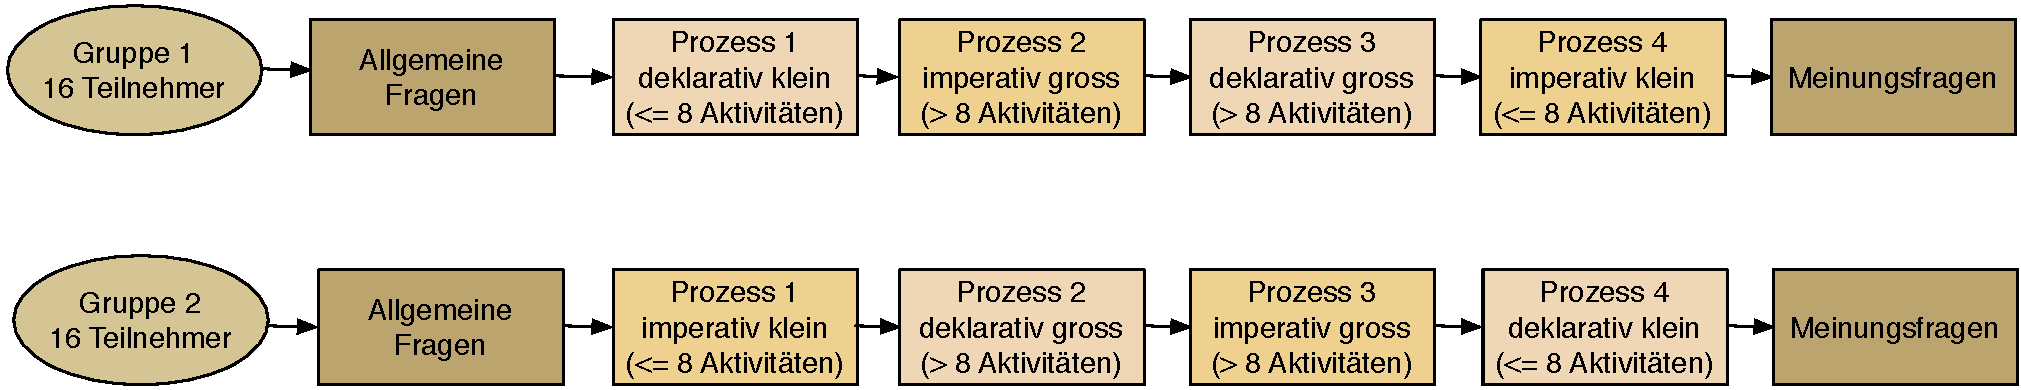
\includegraphics [width=\textwidth]{Umfrage} %pdf, jpg, png...
  \caption{Struktur der Umfrage}
  \label{fig:Umfrage}
\end{center}
\end{figure}

\subsection{Verständnisfragen}

Zu jedem Modell wurden den Teilnehmern jeweils acht Verständnisfragen gestellt. Diese zielten auf das Verständnis der möglichen Reihenfolge der Aktivitäten, mögliche Start- und Endaktivitäten, allgemeine Informationen aus dem Modell sowie parallele Abläufe von Aktivitäten, sich ausschließende Aktivitäten und die Anzahl möglicher Ausführungen von Aktivitäten.\newline
Die Teilnehmer konnten bei der Beantwortung der Fragen zwischen den folgenden vier Antwortmöglichkeiten wählen: \textit{Ja}, \textit{Nein}, \textit{Geht nicht aus Modell hervor} und \textit{Unentschlossen}.

\subsection{Umfragewerkzeug und Durchführung}

Zur Durchführung wurde das Fragebogenwerkzeug \textit{Limesurvey} verwendet. Der entsprechende Link zum Fragebogen sowie eine Legende zur Notationsübersicht von Declare und BPMN wurden den Teilnehmern per E-Mail zugeschickt. Die entsprechenden Antworten der Probanden wurden automatisch von \textit{Limesurvey} gespeichert. Die gespeicherten Daten können aus \textit{Limesurvey} für verschiedene externe Anwendungen exportiert werden (z.B. Excel, CSV oder für SPSS).

\subsection{Auswertung}

Für jede richtige Antwort wurde 1 Punkt vergeben. Für jede falsche Antwort gab es 0 Punkte. Auch \textit{Unentschlossen} wurde als falsche Antwort gewertet. Die einzelnen Punkte wurden dann pro Frage aufsummiert, so dass ein maximaler Wert pro Frage von 1 möglich war.

\section{Durchführung der Studie}

Im Folgenden wird die Durchführung der Studie genau beschrieben.

\subsection{Teilnehmer}

Es wurden 32 Studenten und Doktoranden aus dem Bereich Informatik/Medieninformatik befragt. 12 Teilnehmer waren weiblich und 20 männlich. Die allgemeinen demographischen Daten der Probanden können Abbildung \ref{fig:TabelleAllgemeineDaten} entnommen werden. Diese hatten unterschiedliches Hintergrundwissen zum Thema Prozessmodellierung. Wie Abbildung in \ref{fig:VerteilungImperativDeklarative} zu sehen ist, hatten sieben Studienteilnehmer weder in imperativer noch in deklarativer Modellierung Erfahrung (Teilnehmer, welche angaben seit 0-1 Jahr imperative oder deklarative Prozessmodelle zu modellieren und im letzten Jahr keine imperativen oder deklarativen Prozessmodelle erstellt zu haben). 15 Probanden hatten nur in imperativer Modellierung Erfahrung, jedoch nicht in deklarativer Modellierung (Teilnehmer, die angaben seit mehr als 1 Jahr imperative Prozessmodelle zu erstellen und seit 0-1 Jahr deklarative Prozessmodelle zu erstellen und im letzten Jahr keine deklarativen Prozessmodelle erstellt haben). 10 weitere Teilnehmer hatten in beiden Modellierungssprachen Erfahrung. Die Versuchsobjekte wurden bewusst nach unterschiedlichem Hintergrundwissen zum Thema Prozessmodellierung ausgewählt um zu prüfen, in wie fern sich die Ergebnisse bei den Verständnisfragen zwischen Personen mit viel und wenig Hintergrundwissen zum Thema Prozessmodellierung unterscheiden.\newline


\begin{figure}[htp]
\begin{center}
  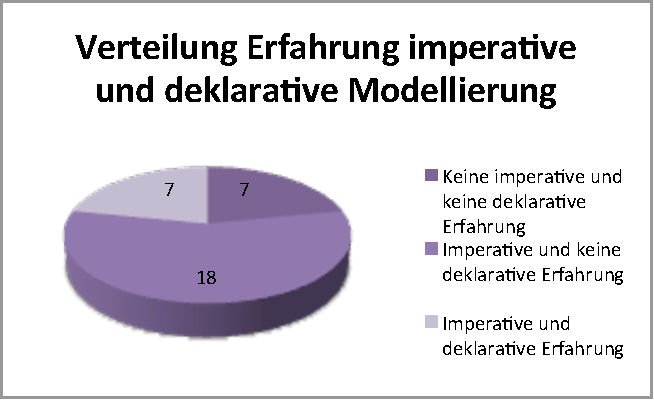
\includegraphics{VerteilungImperativDeklarative} %pdf, jpg, png...
  \caption{Verteilung Erfahrung imperative und deklarative Modellierung}
  \label{fig:VerteilungImperativDeklarative}
\end{center}
\end{figure}

\begin{figure}[htp]
\begin{center}
  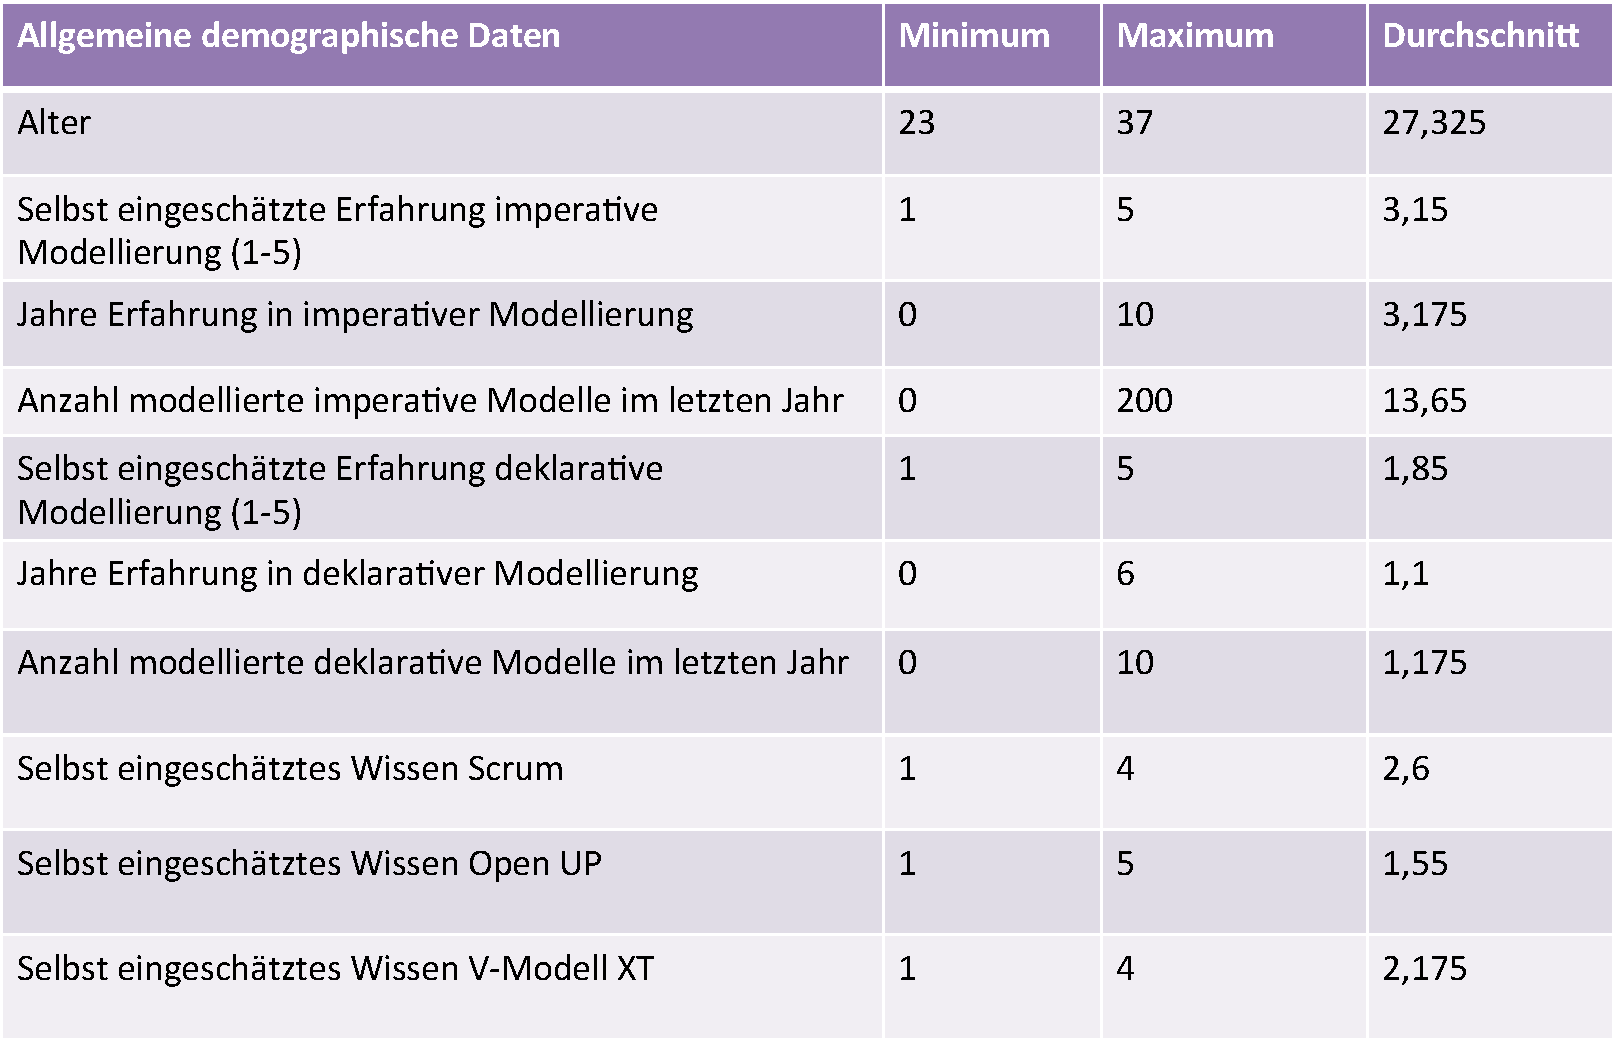
\includegraphics[width=\textwidth]{TabelleAllgemeineDaten} %pdf, jpg, png...
  \caption{Allgemeine demographische Daten}
  \label{fig:TabelleAllgemeineDaten}
\end{center}
\end{figure}



\subsection{Ergebnisse Verständnisfragen}

Abbildung \ref{fig:Frage1} zeigt die Ergebnisse der Verständnisfragen zum Modell \grqq Open UP: Lösungsinkrement entwickeln\grqq. Während die Ergebnisse teilweise gleich sind, bzw. nur wenig voneinander abweichen, liegen die Ergebnisse der deklarativen Modelle bei den Fragen 5 und 6 deutlich unter den Ergebnissen der imperativen Modelle. Diese werden nachfolgend gesondert dargestellt. \newline
Bei Frage 5 (\grqq Nach Ausführung der Aktivität \grqq Integrieren\grqq \ endet der Prozess in jedem Fall sofort\grqq) wurde von den Teilnehmern die imperative XOR- Verknüpfung besser verstanden als die deklarative Darstellung des Ablaufes. Auch bei Frage 6 (\grqq Als erste Aktivität im Prozess kann die Aktivität \grqq Entwickeltest implementieren\grqq \ ausgeführt werden\grqq) war den Probanden die imperative XOR-Darstellung, wohl in Verbindung mit dem BPMN Startsymbol als eindeutigen Einstiegspunkt klarer, als die entsprechende deklarative Darstellung.\newline
Der gesamte Mittelwert aller acht Fragen beträgt bei der imperativen Gruppe 0,96 und bei der deklarativen Gruppe 0,76. Somit ist die Verständnisfrage 1 bei der imperativen Gruppe besser ausgefallen als bei der deklarativen Gruppe. \newline

\begin{figure}[htp]
\begin{center}
  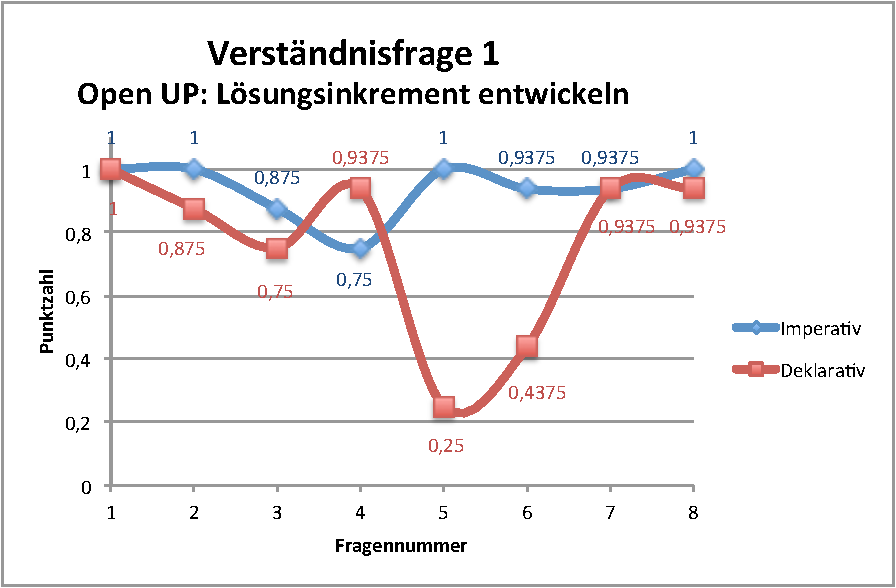
\includegraphics[scale=0.8]{Frage1} %pdf, jpg, png...
  \caption{Ergebnisse Verständnisfrage 1 aller Teilnehmer}
  \label{fig:Frage1}
\end{center}
\end{figure}


Die Ergebnisse der Verständnisfrage 2 zum Modell \textit{Scrum} von allen Teilnehmern kann Abbildung \ref{fig:Frage2} entnommen werden.  Bei Scrum handelte es sich um ein großes Modell (>8 Aktivitäten), welches sowohl viele Verzweigungen als auch viele parallele Aktivitäten aufweist. Auch hier weichen die Ergebnisse der imperativen und deklarativen Modelle voneinander ab.\newline
Nur bei der ersten Frage (\grqq Ein Scrum Meeting dauert 15 Minuten\grqq) schnitt der deklarative Prozess besser ab als der imperative Prozess. Diese allgemeine Information aus dem Prozess befand sich bei beiden Prozessen in der Beschriftung der Aufgabe \grqq 15-minütiges Scrum Meeting durchführen\grqq. Der imperative Scrum-Prozess weist insgesamt mehr Elemente auf als der deklarative Scrum-Prozess. Daher fiel es wohl den Probanden leichter, die Übersicht über allgemeine Informationen zu behalten.\newline
Bei den Fragen 2 und 8 hat das deklarative Modell eine sehr schlechte Punktzahl erreicht. Bei Frage 2 (\grqq Die Aktivität \grqq Task abarbeiten\grqq \ kann beliebig ausgeführt werden\grqq) konnten die Teilnehmer der XOR-Verknüpfung im imperativen Modell, welche eine Rückschleife auf die Aktivität \grqq Task abarbeiten\grqq, besser folgen als der entsprechenden Darstellung der Aktivität im deklarativen Modell. \newline
Das Gleiche gilt für Frage 8 (\grqq Nach Beendigung der Aufgabe \grqq Task abarbeiten\grqq \ endet der Prozess sofort\grqq). Auch hier wurde die Verzweigung und das damit mögliche Zurückkehren zur Aufgabe \grqq Sprint-Planning-Meeting durchführen\grqq \ durch eine XOR-Verknüpfung im imperativen Modell dargestellt und war somit für die Teilnehmer klarer verständlich.\newline
Der Mittelwert aller acht Fragen insgesamt ist bei der imperativen Gruppe 0,89 und bei der deklarativen Gruppe 0,70. Die Fragen wurden also von der imperativen Gruppe richtiger beantwortet als von der deklarativen Gruppe.\newline


\begin{figure}[htp]
\begin{center}
  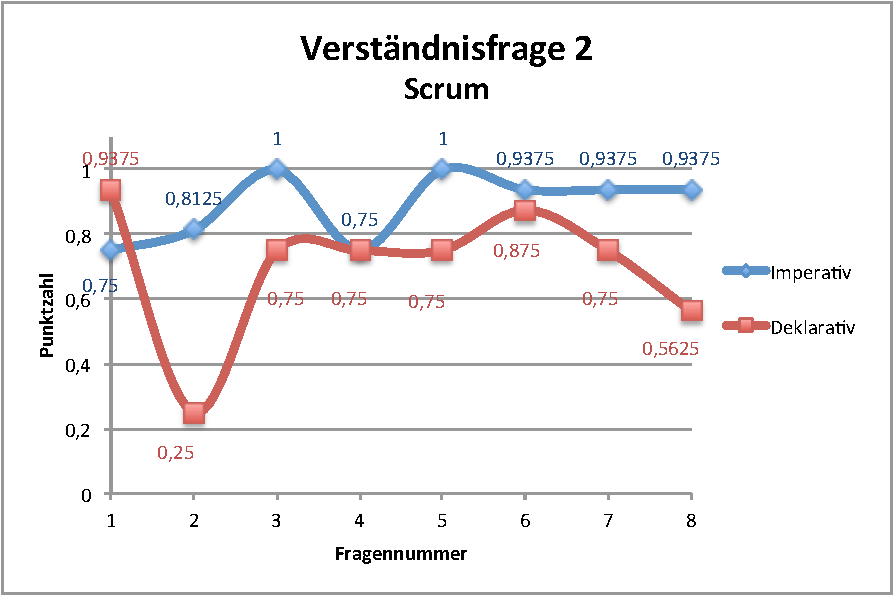
\includegraphics[scale=0.8]{Frage2} %pdf, jpg, png...
  \caption{Ergebnisse Verständnisfrage 2 aller Teilnehmer}
  \label{fig:Frage2}
\end{center}
\end{figure}

Beim Modell \grqq V-Modell: Systementwicklungsprojekt AG/AN\grqq \ der Verständnisfrage 3 lagen die Ergebnisse des deklarativen Modell bis auf Frage 3 immer unter denen des imperativen Modells (Abbildung \ref{fig:Frage3}). Starke Abweichung gab es bei den Fragen 2, 4, 5, 6 und 7. \newline
Bei Frage 2 (\grqq Die Aktivitäten \grqq Prototypische Entwicklung durchführen\grqq, \grqq Komponentenbasierte Entwicklung durchführen\grqq \ und \grqq Inkrementelle Entwicklung durchführen\grqq \ können parallel zueinander ausgeführt werden\grqq) war den Teilnehmern, welche das deklarative Modell bearbeiten mussten, die Notation des Constraints \textit {Exclusive Choice 1 of 3} nicht ganz klar. Sechs der 16 Probanden kreuzten hier entweder \textit{Ja} oder \textit{Unentschlossen} an. Es musste im deklarativen Modell ein zusätzlicher Unterprozess eingefügt werden da das Verhalten des Prozesses nicht anders darzustellen war. Eventuell waren die Probanden auch von dem zusätzlichen Unterprozess irritiert.\newline
Frage 4 (\grqq Nach Ausführung der Aktivität \grqq System abnehmen\grqq \ kann die Aktivität \grqq Anforderungen festlegen\grqq \ ausgeführt werden\grqq \ und Frage 5 (\grqq Nach Ausführung der Aktivität \grqq System abnehmen\grqq \ kann die Aktivität \grqq Projekt ausschreiben\grqq \ ausgeführt werden\grqq) zielten wieder auf Verzweigungen des Prozesses ab. Der imperative Prozess war den Teilnehmern verständlicher. \newline
Frage 6 (\grqq Die Aktivität "Iteration planen" kann innerhalb einer Prozessinstanz genau einmal ausgeführt werden\grqq) wurde von der deklarativen Gruppe weniger richtig beantwortet als von der deklarativen. Es war der deklarativen Gruppe vermutlich die Möglichkeit zur Rückkehr an eine frühere Aktivität im Prozess nicht ganz klar. \newline
Frage 7 (\grqq Nach Ausführung der Aktivität \grqq Projekt abschließen\grqq \ endet der Prozess\grqq) wurde von den Probanden, welchen das imperative Modell gezeigt wurde, richtiger beantwortet. Hier war im imperativen Modell durch das BPMN-Ende-Symbol den Teilnehmern das Ende des Prozesses wohl bewusster als die Darstellung durch das Constraint \textit{not succession} im deklarativen Modell.\newline
Bei allen acht Fragen insgesamt ist der Mittelwert bei der imperativen Gruppe 0,94 und bei der deklarativen Gruppe 0,67. Demnach wurden die Modelle von der imperativen Gruppe deutlich besser verstanden als von der deklarativen Gruppe. \newline


\begin{figure}[htp]
\begin{center}
  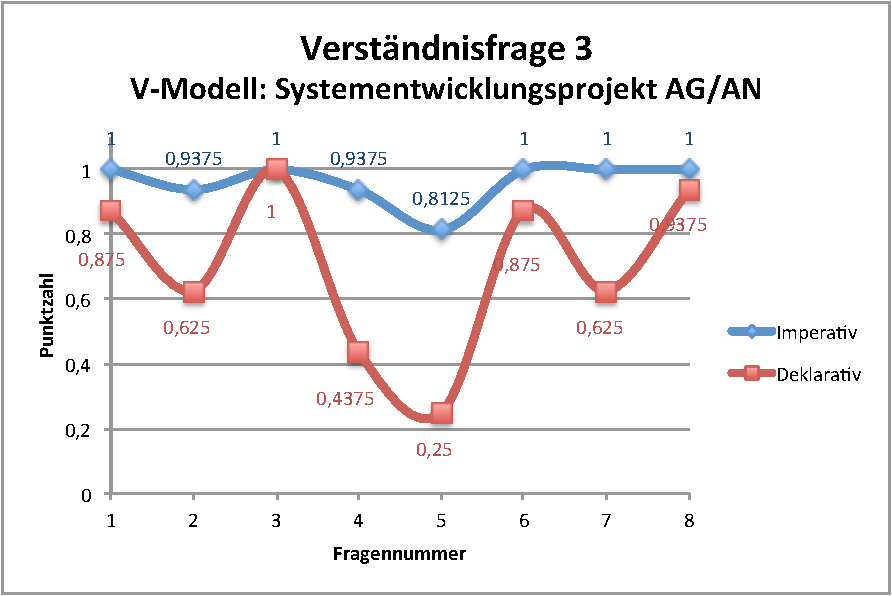
\includegraphics[scale=0.8]{Frage3} %pdf, jpg, png...
  \caption{Ergebnisse Verständnisfrage 3 aller Teilnehmer}
  \label{fig:Frage3}
\end{center}
\end{figure}

Die Ergebnisse des Prozesses \grqq Open UP: Inception\grqq \ weichen zwischen den deklarativen und imperativen Modellen nicht stark voneinander ab (Abbildung \ref{fig:Frage4}). \newline
Lediglich bei Frage 6 (\grqq Die Aktivität \grqq Iteration planen und managen\grqq \ kann beliebig oft ausgeführt werden\grqq) und Frage 7 (\grqq Die Aktivitäten \grqq Anforderungen identifizieren und verfeinern\grqq \ und \grqq auf technisches Vorgehen einigen\grqq \ können beliebig oft ausgeführt werden) war den Teilnehmern offenbar teilweise die Funktion des Existenz Constraints nicht ganz klar oder wurde übersehen.\newline
Der Mittelwert aller acht Fragen beträgt bei der imperativen Gruppe 0,96 und bei der deklarativen Gruppe 0,87. Hier wurden die Modelle von der imperativen Gruppe besser verstanden als von der deklarativen Gruppe. \newline


\begin{figure}[htp]
\begin{center}
  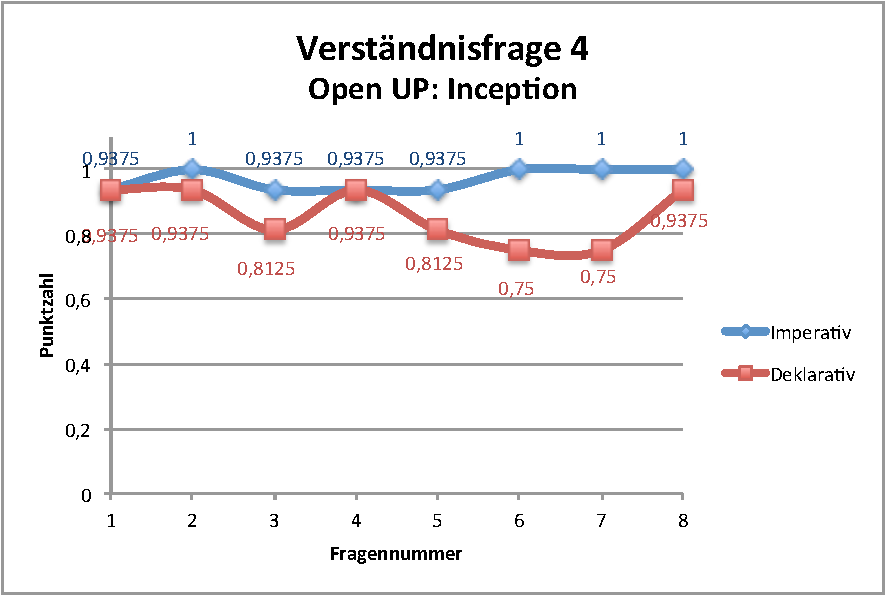
\includegraphics[scale=0.8]{Frage4} %pdf, jpg, png...
  \caption{Ergebnisse Verständnisfrage 4 aller Teilnehmer}
  \label{fig:Frage4}
\end{center}
\end{figure}

In Abbildung \ref{fig:TabelleAufg} können die Mittelwerte der vier Verständnisfragen aufgeteilt nach der Erfahrung der Teilnehmer eingesehen werden. Hier lässt sich erkennen, dass die Ergebnisse zu den deklarativen Modellen von Teilnehmern mit deklarativer Modellierungserfahrung über dem Durchschnitt liegen, während sie bei den beiden Gruppen ohne deklarative Erfahrung unter dem Durchschnitt liegen. \newline
Bei den Ergebnissen fällt auf, dass die Gruppe, welche weder über imperative noch über deklarative Erfahrung verfügte bei den imperativen Modellen bis auf Verständnisfrage 3 im Durchschnitt liegt. Bei Betrachtung der Werte ist zu beachten, dass sich die Teilnehmerzahlen hier zwischen Gruppe 1 und Gruppe 2 unterscheiden.\newline
\begin{figure}[htp]
\begin{center}
  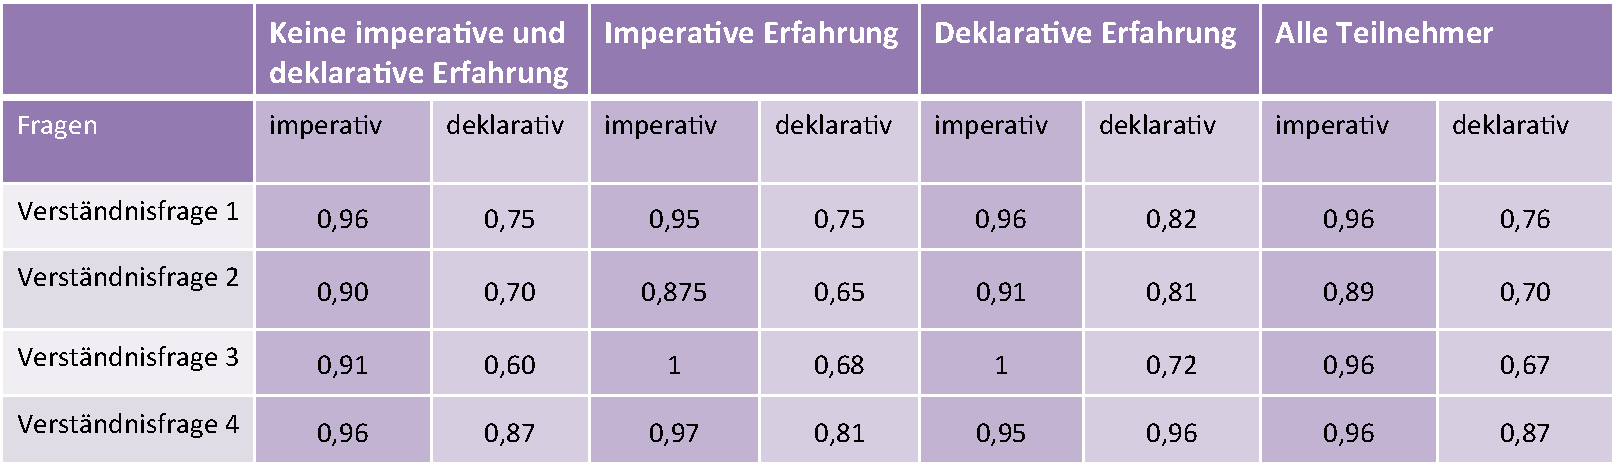
\includegraphics[width=\textwidth]{TabelleAufg} %pdf, jpg, png...
  \caption{Übersicht Ergebnisse der Teilnehmer aufgeteilt nach Erfahrung}
  \label{fig:TabelleAufg}
\end{center}
\end{figure}




\subsection{Ergebnisse Meinungsfragen}

Abbildung \ref{fig:Meinungsfrage1} zeigt, dass 31 der 32 Befragten beim Modell\grqq System spezifizieren\grqq \ das imperative Modell bevorzugen. Nur eine Person zog das deklarative Modell vor. Hierbei handelt es sich um einen Teilnehmer, welcher weder in imperativer, noch in deklarativer Prozessmodellierung Erfahrung hat. Als Begründung für den Vorzug des deklarativen Modells gab der Befragte an, das Modell sei kompakter, jedoch sei auch mehr Verständnis notwendig.\newline
Die Probanden, welche das imperative Modell bevorzugten, gaben verschiedene Gründe hierfür an. Unter anderem nannten sie als Grund die klarere Struktur des BPMN-Modells, die vielen unterschiedlichen/komplexen Elemente im deklarativen Modell oder auch die klare Rollenverteilung durch die Swimlanes. Einige der Befragten gaben auch ihre besseren Kenntnisse in imperativen Prozessmodellierungssprachen als Grund an.\newline

\begin{figure}[htp]
\begin{center}
  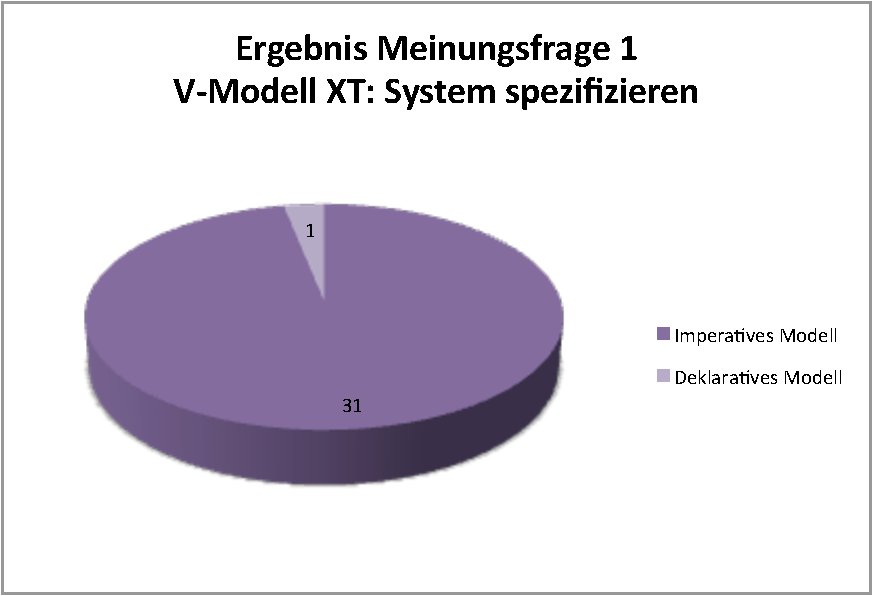
\includegraphics[scale=0.8]{Meinungsfrage1} %pdf, jpg, png...
  \caption{Ergebnisse Meinungsfrage 1 aller Teilnehmer}
  \label{fig:Meinungsfrage1}
\end{center}
\end{figure}

Ebenfalls beim Modell \grqq Phasen Open UP\grqq \ bevorzugt eine deutliche Mehrheit (26 von 32 Befragten) das imperative Modell, wie Abbildung \ref{fig:Meinungsfrage2} entnommen werden kann. \newline
Hierbei verfügte nur einer der sechs Personen, welche das deklarative Modell bevorzugte auch über Erfahrung in deklarativer Modellierung. Die anderen Probanden hatten entweder über keine Erfahrungen in beiden Modellierungssprachen (zwei) oder nur über Erfahrungen in imperativer Modellierung (drei). Als Grund für ihre Wahl gaben die Probanden an, dass das deklarative Modell kompakter sei und dass es klarer sei, dass nur bei Erfolg die nächste Aktivität ausgeführt wird.\newline
Die Personen, welche das imperative Modell präferierten, erklärten, dass sie den Ablauf mit den Schleifen im imperativen Modell klarer finden und dass sie dem Sequenzfluss besser folgen könnten.\newline


\begin{figure}[htp]
\begin{center}
  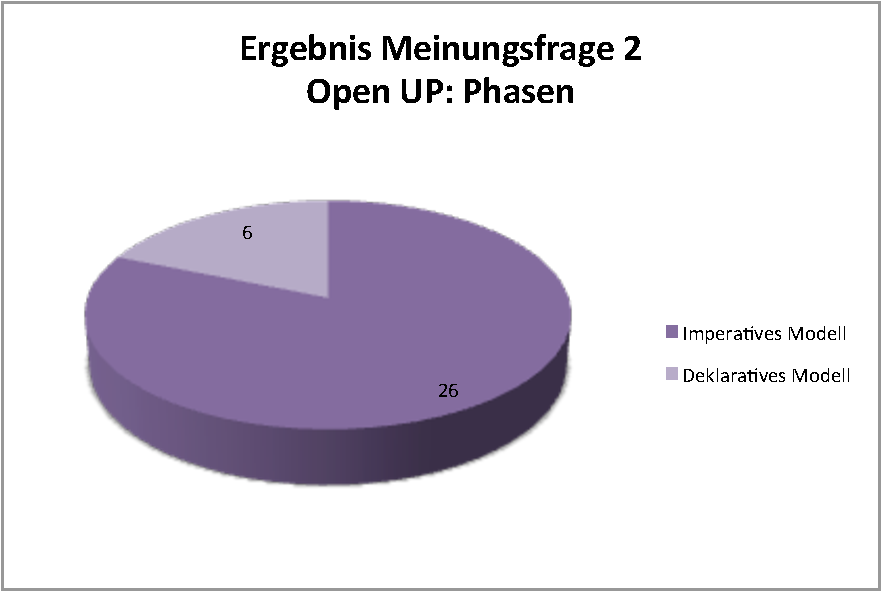
\includegraphics[scale=0.8]{Meinungsfrage2} %pdf, jpg, png...
  \caption{Ergebnisse Meinungsfrage 2 aller Teilnehmer}
  \label{fig:Meinungsfrage2}
\end{center}
\end{figure}

Die Ergebnisse des dritten Modellpaares \grqq Inkrementelle Entwicklung\grqq \ zeigt Abbildung \ref{fig:Meinungsfrage3}. Demnach präferierten nur zwei Personen (eine Person mit Erfahrung sowohl in imperativer als auch in deklarativer Modellierung, eine Person ohne imperative und deklarative Modellierungserfahrung) das deklarative Modell und 30 Probanden ziehen das imperative Modell vor.\newline
Als Grund für den Vorzug des imperativen Modells wurde die Menge an unterschiedlichen Symbolen beim deklarativen Modell genannt. \newline
Die 30 Personen, welchen das imperative Modell besser gefiel, gaben an, dass sie die imperative Notation verständlicher finden. Der Ablauf im imperativen Modell sei klarer erkennbar, sie hätten keinen Anhaltspunkt wo im deklarativen Modell gestartet bzw. geendet wird. Weiterhin würden es die vielen verschiedenen Constraints im deklarativen Modell erschweren den Ablauf nachzuvollziehen.\newline

\begin{figure}[htp]
\begin{center}
  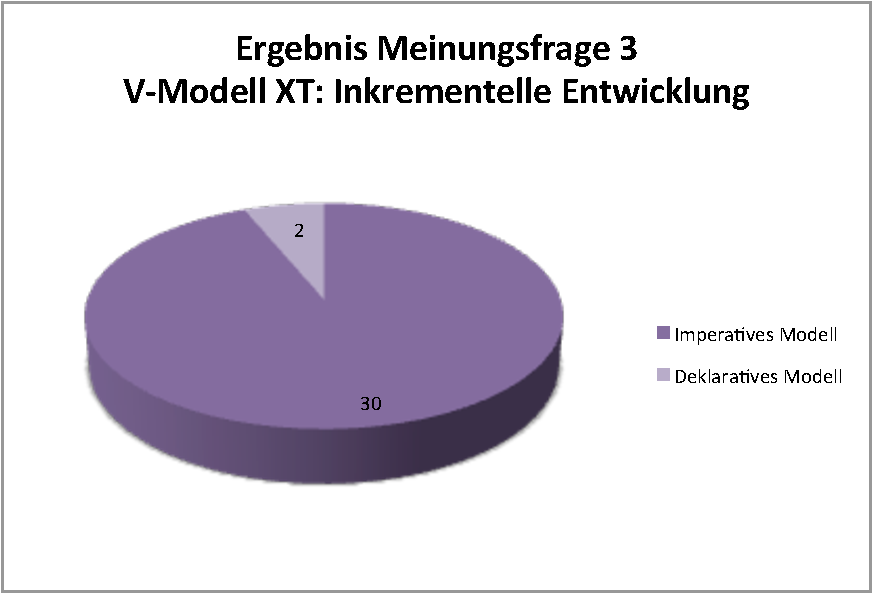
\includegraphics[scale=0.8]{Meinungsfrage3} %pdf, jpg, png...
  \caption{Ergebnisse Meinungsfrage 3 aller Teilnehmer}
  \label{fig:Meinungsfrage3}
\end{center}
\end{figure}

Beim Modell \grqq Open UP: Release deployen\grqq \ präferierten neun Personen das deklarative Modell und 23 Teilnehmer das imperative Modell (Abbildung \ref{fig:Meinungsfrage4}). Von den neun Teilnehmern, welche das deklarative Modell bevorzugten hatte nur einer Kenntnisse in deklarativer Modellierung, einer hatte weder in deklarativer noch in imperativer Modellierung Erfahrung und sieben verfügten nur über Wissen in imperativer Modellierung. \newline
Als Begründung für die Wahl des deklarativen Modelles wurde die Übersichtlichkeit desselbigen genannt und zwar auf Grund der fehlenden Artefakte im Modell. Es wurde bemängelt, dass die vielen Artefakte das imperative Modell unübersichtlich machen würden.\newline
Die Probanden, die das imperative Modell besser fanden, gaben als Gründe den klaren Anfang und das klare Ende des Prozesses an, die bessere Verständlichkeit der Optionalität der Aktivität \textit{Backoutplan ausführen} und die fehlenden Artefakte im deklarativen Modell. \newline



\begin{figure}[htp]
\begin{center}
  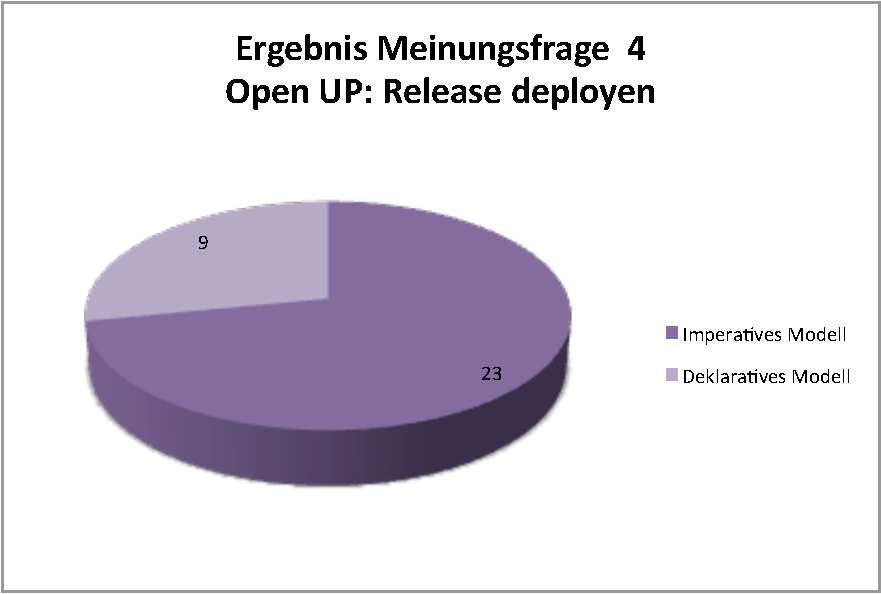
\includegraphics[scale=0.8]{Meinungsfrage4} %pdf, jpg, png...
  \caption{Ergebnisse Meinungsfrage 4 aller Teilnehmer}
  \label{fig:Meinungsfrage4}
\end{center}
\end{figure}


\clearpage

\section{Fazit der Studie}

Durch die Studie konnten die Ergebnisse des Vergleichs aus Kapitel 5 größtenteils belegt werden. Im Folgenden werden die Ergebnisse im Hinblick auf die Forschungsfragen aus Kapitel 6.1 analysiert.\newline

\subsubsection{Richtigkeit, Relevanz}


In den Modellen \grqq Scrum (Verständnisfrage 2)\grqq, \grqq System spezifizieren (Meinungsfrage 1)\grqq \ und \grqq Release deployen (Meinungsfrage 4)\grqq \ waren sowohl Artefakte, als auch Rollen enthalten. Die Differenz der Punktsummen zwischen der imperativen und der deklarativen Gruppe von \grqq Scrum\grqq \ beträgt 0,1875. Dies ist die zweitgeringste Abweichung zwischen der imperativen und der deklarativen Gruppe. Zwei Modelle, bei denen auch im imperativen Modell keine Rollen und Artefakte abgebildet waren, hatten sogar noch größere Differenzen zwischen der imperativen und der deklarativen Gruppe. Aus diesem Grund kann hier kein besseres Verständnis des Prozessablaufes durch Rollen und Artefakte angenommen werden [A 1.2], [A 3.1]. \newline
Die fehlende Visualisierbarkeit von Rollen im deklarativen Modell wurde von keinem der Teilnehmer bemängelt im Zuge der Meinungsfragen.\newline



\subsubsection{Systematischer Aufbau}

Wie bereits beim Grundsatz Richtigkeit erwähnt, kann kein negativer Einfluss auf die Verständlichkeit beobachtet werden wenn im deklarativen Modell keine Artefakte enthalten sind.\newline
Während ein großer Teil der Probanden bei den Modellen \grqq System spezifizieren (Meinungsfrage 1)\grqq \ und \grqq Release deployen (Meinungsfrage 4)\grqq \ fehlende Artefakte im deklarativen bemängelten, empfand ein kleiner Teil der Probanden diese im imperativen Modell als störend. Die Mehrheit der Teilnehmer entschied sich jedoch für das imperative Modell mit der Begründung, dass die Artefakte beim Verständnis helfen würden [A 2.1]. 

\subsubsection{Klarheit, Wirtschaftlichkeit}



Nachfolgend werden die beiden Grundsätze \textit{Klarheit} und \textit{Wirtschaftlichkeit} zusammengefasst, da sie hier die gleichen Kriterien haben und die \textit{Wirtschaftlichkeit} im Rahmen dieser Studie nicht getestet werden kann.\newline

Bei Modellen mit vielen Verzweigungen bzw. Schleifen war für die Teilnehmer BPMN verständlicher. Dies zeigte sich beim kleinen (<= 8 Aktivitäten) Prozess \grqq Open UP: Lösungsinkrement entwickeln\grqq, bei dem die Punktzahlen bei der BPMN Gruppe leicht höher waren und noch deutlicher als beim großen Modell (> 8 Aktivitäten) \grqq V-Modell: Systementwicklungsprojekt AG/AN\grqq. Bei diesen beiden Prozessen sind in ConDec deutlich mehr Constraints notwendig als Gateways in BPMN, vor allem werden viele verschiedene Constraints zur korrekten Darstellung des Ablaufs benötigt. Dadurch haben die ConDec-Modelle eine deutlich höhere Komplexität als die BPMN-Modelle [A 4.1], [A 4.3].\newline

Es fällt besonders auf, dass Fragen bezüglich der Reihenfolge der Aktivitäten bei ConDec bei direkt aufeinander folgenden Aktivitäten größtenteils richtig beantwortet wurden. Jedoch bei Abläufen, bei denen es durch Verzweigungen im Prozessablauf zu einem Rücksprung kommt, wurden nur die Fragen zu den BPMN-Modellen größtenteils richtig beantwortet. Bei ConDec wurden diese Fragen häufig falsch beantwortet [A 4.1], [A 4.3].\newline

Das gleiche gilt für den großen Prozess (> 8 Aktivitäten) \grqq Scrum\grqq. Die beiden Fragen, welche von der deklarativen Gruppe sehr fehlerhaft verstanden wurden, hatten beide mit Verzweigungen innerhalb des Prozesses zu tun und wurden von der imperativen Gruppe durch die dortige Darstellung mit Hilfe eines XOR-Gateways wesentlich besser verstanden. Jedoch konnte die allgemeine Frage zum Prozess wie lange ein Scrum-Meeting dauert, von der deklarativen Gruppe besser beantwortet werden. Da der deklarative Prozess über weniger Elemente verfügt als der imperative und somit kompakter ist, können allgemeine Informationen leichter gefunden werden [A 4.1], [A 4.3]. \newline
Beim letzten Prozess \grqq Inception\grqq \ haben sich die Erkenntnisse aus Kapitel 5 nicht ganz bestätigt. Auf Grund der vielen parallelen Aktivitäten in diesem Prozess ist der deklarative Prozess hier der weniger komplexe und übersichtlichere. Jedoch wurden die Modelle von der imperativen Gruppe dennoch häufiger besser verstanden. Zwar ist der Unterschied nicht sehr groß, dennoch war hier das Ergebnis genau gegensätzlich erwartet [A 4.1], [A 4.3].\newline
Die Fragen nach der ersten auszuführenden Aktivität im Modell fielen bei den deklarativen Gruppen, bei den Modellen ohne klaren Einstiegspunkt leicht schlechter aus, als bei den imperativen Gruppen, bei denen es im Modell durch das Startzeichen stets einen klaren Einstiegspunkt gab [A 4.2]. \newline

Bei den Meinungsfragen wurden bei allen Modellen die imperativen Prozesse vorgezogen. Die Begründungen der Teilnehmer bestätigen größtenteils die Ergebnisse aus Kapitel 5. Viele Teilnehmer gaben die hohe Komplexität der ConDec Constraints an, vor allem bei den Modellen \grqq System spezifizieren\grqq \ und \grqq Inkrementelle Entwicklung\grqq. In diesen beiden Modellen finden sich sehr viele (auch unterschiedliche) Constraints, was die Modelle sehr komplex macht [A 4.1], [A 4.3].\newline
Bei den beiden Modellen \grqq Open UP: Phasen\grqq \ und \grqq Release deployen\grqq \ wurden als Grund hauptsächlich die bessere Verständlichkeit der Schleifen/Optionalitäten von Aufgaben genannt. Diese wurden in den imperativen Modellen mit XOR-Verbindungen dargestellt, anstelle von mehreren Constraints bei den ConDec Modellen. Auch hier zeigt sich wieder, dass die BPMN-Modelle bei Prozessen mit Schleifen/Verzweigungen weniger komplex sind als die ConDec Modelle und daher auch besser verständlich sind [A 4.1], [A 4.3].\newline
Aus Abbildung \ref{fig:TabelleAufg} lässt sich erkennen, dass es für Personen ohne Modellierungserfahrung offensichtlich einfacher ist, imperative Modelle zu verstehen, da deren Ergebnisse bei den imperativen Modellen im Durchschnitt liegen und sich bei den deklarativen Modellen unter dem Durchschnitt befinden. Personen mit deklarativer Erfahrung liegen hingegen bei den deklarativen Modellen über dem Durchschnitt.\newline



\subsubsection{Vergleichbarkeit}
Das gleiche Ausführungsverhalten der deklarativen und imperativen Prozesse wurde schon im Zuge der Vergleiche aus Kapitel 5 getestet und sichergestellt [A 6.1]. \newline
Obwohl bei manchen Modellen die BPMN-Modelle insgesamt mehr Elemente aufweisen, weisen die imperativen Gruppen dennoch grundsätzlich höhere Punktzahlen auf als die deklarativen Gruppen. Einzig beim Modell \grqq Scrum\grqq \ wurde die allgemeine Frage zum Prozess, wie lange ein Scrum-Meeting dauern würde, von der deklarativen Gruppe besser beantwortet als von der imperativen Gruppe. Dennoch kann hier den größeren BPMN-Modellen keine mangelnde Vergleichbarkeit zugeschrieben werden [A 6.2].\newline
Bei ConDec gibt es hier wiederum Grenzen in der Darstellbarkeit in Bezug auf Rollen und Artefakte, weshalb ConDec an dieser Stelle die Vergleichbarkeit nicht einhalten kann [A 6.3].\newline


Tabelle \ref{fig:TabelleStudie} fasst die Ergebnisse der Studie nochmal zusammen:

\begin{figure}[htp]
\begin{center}
  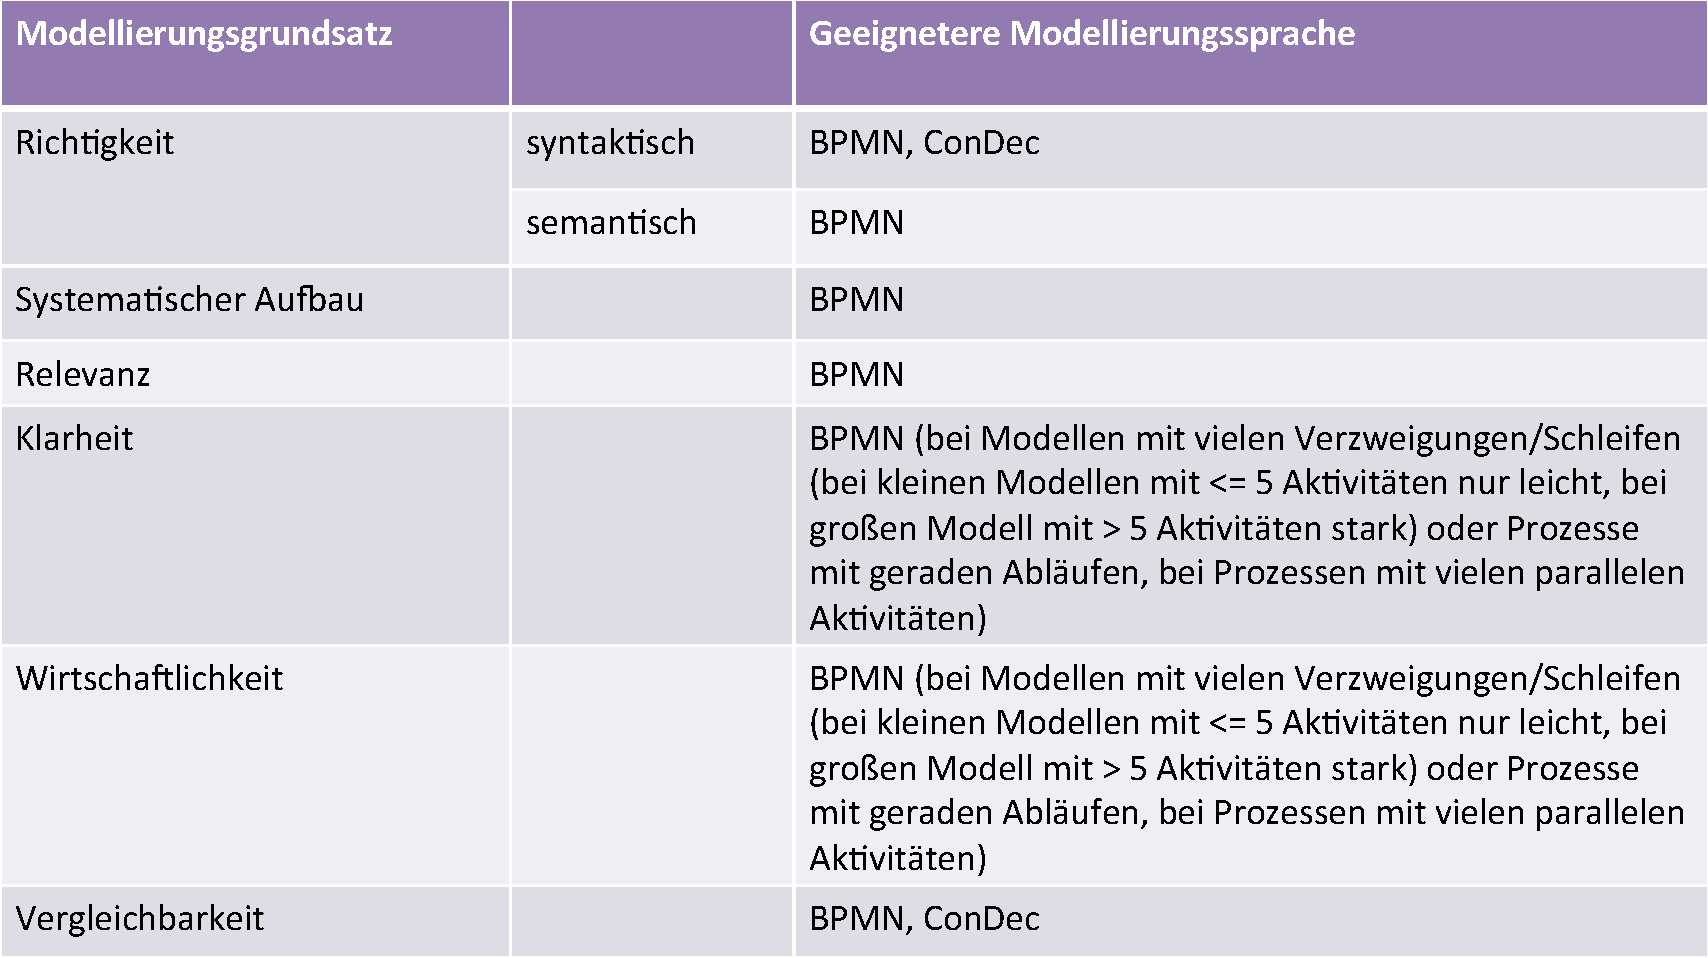
\includegraphics[width=\textwidth]{TabelleStudie} %pdf, jpg, png...
  \caption{Zusammenfassung Ergebnisse Studie}
  \label{fig:TabelleStudie}
\end{center}
\end{figure}

Die kompletten Rohdaten der Umfrage mit allen Antworten der Teilnehmer können Anhang D entnommen werden. Die kompletten Fragebögen von Gruppe 1 und Gruppe 2 können Anhand C entnommen werden.\newline

\subsection{Grenzen der Studie}

Eine große Menge der Teilnehmer hatte einige Vorkenntnisse in imperativer Modellierung (15 nur imperativ, 10 imperativ und deklarativ). Einige der Befragten gaben auch bei den Meinungsfragen an, sie hätten einfach bessere Kenntnisse in imperativer Modellierung und würden daher die imperativen Modelle bevorzugen. Aus diesem Grund kann hier ein Einfluss der besseren Kenntnis der imperativen Modellierung der Probanden auf die Ergebnisse der Studie nicht ausgeschlossen werden. \newline 
Zudem konnten die Ergebnisse von Personengruppen ohne jegliche imperative und deklarative Prozessmodellierungserfahrung und Personengruppen mit imperativer oder imperativer und deklarativer Prozessmodellierungserfahrung nur begrenzt miteinander verglichen werden, da sich die Zahl dieser Personengruppen stark voneinander unterschied (7 gegen 15 gegen 10 Personen).\newline
Weiterhin wurde zwar darauf geachtet, Modelle mit unterschiedlichen Abläufen und Größen auszuwählen, jedoch können die Ergebnisse trotzdem nicht unbedingt grundsätzlich auf alle imperativen und deklarativen Modellpaare übertragen werden. \newline

 












